\scanpage{72}
\mspage{\handwritten{\raisebox{0.65ex}{-}\,7\,-}}

page 25, line 10 from the bottom : hint for ``it is not difficult to show ...''?

page 26, line 10 : ``which one may think is the same ...'' : is there
\figure{%
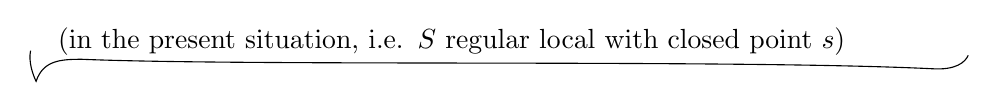
\begin{tikzpicture}
\node[anchor=south west,inner sep=0pt,outer sep=0pt,text width=0.94\linewidth,align=left] (addition) at (0,0) {\inserted{(in the present situation, i.e. $S$ regular local with closed point $s$)}};
\handwritten{\draw[line width=0.4pt]
 ([xshift=-3.5mm,yshift=0.6mm]addition.south west)
 .. controls ([xshift=-3.8mm,yshift=-0.8mm]addition.south west)
 and ([xshift=-3.2mm,yshift=-2.5mm]addition.south west)
 .. ([xshift=-2.8mm,yshift=-3.3mm]addition.south west)
 .. controls ([xshift=-1.9mm,yshift=-0.6mm]addition.south west)
 and ([xshift=0.4mm,yshift=-0.5mm]addition.south west)
 .. ([xshift=3.0mm,yshift=-0.5mm]addition.south west)
 .. controls ([xshift=25mm,yshift=-1.4mm]addition.south west)
 and ([xshift=-28mm,yshift=-0.5mm]addition.south east)
 .. ([xshift=-3mm,yshift=-1.7mm]addition.south east)
 .. controls ([xshift=0mm,yshift=-1.9mm]addition.south east)
 and ([xshift=1.2mm,yshift=-0.9mm]addition.south east)
 .. ([xshift=1.6mm,yshift=0mm]addition.south east);}
\end{tikzpicture}%
}
\noindent a characterization of a homomorphism (7.17.4.1) ? \handwritten{(${}^1$)}

page 27, lines 1 and 2 from the bottom : ``above'' and not ``above''. Say ``in the normalization'' instead of ``of the normalization''.

page 28 : in the bibliography, the Abhyankar reference on the resolution of singularities
of arithmetic surfaces is missing.

\handwritten{(${}^1$) Does 7.2 not \unsure{x|itself} generalize ?}

% Detached dark marks in the lower-right blank area; authored status and function uncertain.
\par\vspace*{0.27\textheight}
\noindent\hfill\parbox[c]{3mm}{\figure{\unsure{%
\begin{tikzpicture}[x=1mm,y=1mm]
\fill (-0.39,-0.02) .. controls (-0.44,0.18) and (-0.23,0.27) .. (-0.17,0.45)
 .. controls (0.01,0.59) and (0.15,0.29) .. (0.23,0.19)
 .. controls (0.48,0.13) and (0.43,-0.09) .. (0.19,-0.18)
 .. controls (0.05,-0.40) and (-0.17,-0.29) .. (-0.39,-0.02) -- cycle;
\fill (0.58,1.30) .. controls (0.66,1.49) and (0.84,1.48) .. (0.89,1.73)
 .. controls (0.97,1.93) and (1.13,1.72) .. (1.14,1.58)
 .. controls (1.32,1.44) and (1.25,1.24) .. (1.10,1.16)
 .. controls (1.01,0.97) and (0.75,1.08) .. (0.58,1.30) -- cycle;
\fill (-0.60,1.38) ellipse[x radius=0.15,y radius=0.16];
\end{tikzpicture}%
}}}\hspace*{0.04\linewidth}\par

% archive sheet number: 71
\clearpage
